\documentclass{article}
%\usepackage{fullpage}
\usepackage{fancyhdr}
\usepackage[english,francais]{babel}
\usepackage[T1]{fontenc}
\usepackage[utf8]{inputenc}
\usepackage[pdftex]{graphicx}
\usepackage{subfig}

%\renewcommand{\baselinestretch}{2}
\author{Florent \textsc{Guiotte} et Frédéric \textsc{Becker}}
\title{Ray tracing}
\pagestyle{fancy}

\begin{document}
\maketitle
\tableofcontents

\section{Introduction}

L'objectif de ce TP est d'écrire la méthode qui retourne la couleur à dessiner sur une image dans un projet de ray tracing.
Nous nous occupons donc d'implémenter les algorithmes de lancé de rayons\footnote{Les algorithmes sont issus des cours de
    Kadi \textsc{Bouatouch}, notamment ceux du modèle de \textsc{Phong}, la réflectance\ldots} avec comme paramètres un vecteur représentant
le rayon à lancer à travers la scène, une liste de géométries représentant les objets (entièrement composés de
triangles, associé à un matériau) et de la liste des lumières de la scène. Notre méthode sera appelée pour chaque pixel
de l'image.

Pour réaliser ce TP, nous avons utilisé le projet et plusieurs classes/objets issus du logiciel de raytracing développé par
Fabrice \textsc{Lamarche}.

%\begin{figure}[!ht]%htp]
%  \centering
%  \subfloat[Image d'origine]{\label{fig:loup}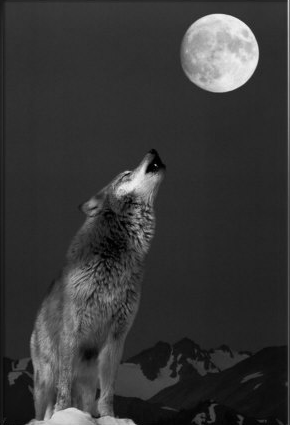
\includegraphics[width=0.48\textwidth]{img/loup.png}}
%  \hspace{0.030\textwidth}
%  \subfloat[Gradient de l'image]{\label{fig:gradient}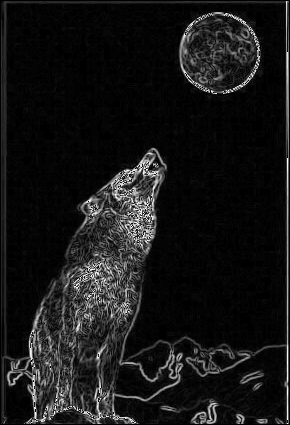
\includegraphics[width=0.48\textwidth]{img/energie.png}}
%  \caption{Loup.pgm et calcul de l'énergie associée}
%  \label{fig:init}
%\end{figure}


\section{Détail de l'algorithme}
\subsection{Intersection}

Le premier calcul à faire est de trouver l'intersection la plus proche de la caméra entre le rayon émis de cette
dernière et le triangle d'un objet qui compose la scène (si l'intersection existe). 

Nous avons implémenté une méthode qui permet d'obtenir l'intersection la plus proche de la source d'émission du rayon
et la scène afin d'alléger la méthode \textit{sendRay} et pour la réutiliser un peu plus loin pour les
ombres\footnote{partie \ref{ombre} page \pageref{ombre}}. Cette méthode parcours les triangles qui composent les objets
de la scène, et détecte s'il y à intersection. Si c'est le cas, on la conserve pour pouvoir la comparer si une nouvelle
intersection est trouvée. En effet, afin d'avoir le rendu de la face visible à l'écran, il ne faut prendre en compte que
celle qui est la plus proche de la caméra, les autres seront <<cachées>> par cette face, donc n'ont pas besoin d'être
dessinées. Techniquement, nous utilisons juste une \textit{intersection} en cache afin de la comparer avec la nouvelle, et de
conserver la plus proche des deux (plutôt que d'utiliser un Z-buffer par exemple).

Si il n'y a aucune intersection entre le rayon et la scène, alors on renvois une couleur par défaut (couleur de fond).

\subsection{Ombrage}
\label{ombre}

Avant d'appliquer le modèle de \textsc{Phong}, il faut vérifier que l'intersection est éclairée par une lampe.
On parcours les lampes de la scène, pour chacune d'entre elle on créé le rayon qui part de la lampe dans la direction de l'intersection trouvée
précédemment. On l'appellera rayon d'ombrage.

Il suffit de rappeler la méthode décrite précédemment pour trouver l'intersection la plus proche de la lampe. Si le
triangle correspondant à l'intersection de ce rayon d'ombrage est le même que celui qui correspond à
l'intersection trouvée dans la première partie, c'est que ledit triangle est éclairé par cette lumière.

\subsection{Phong}

Lors du parcours des lampes de la scènes, si le triangle correspondant à l'intersection est éclairé par une lampe, alors
on applique les calculs du modèle de \textsc{Phong} qui gèrent de manière réaliste l'intensité d'éclairage d'une
surface.

Les calculs se décomposent en deux parties, le calcul de l'éclairage diffus de la surface et le calcul du reflet
spéculaire  (tache lumineuse, reflet d'une source de lumière dans l'objet). 

Le calcul du diffus prend en paramètre un
vecteur \textit{Kd} qui est renseigné dans le matériau du triangle (il représente une couleur) à laquelle on multiplie
l'intensité de la lumière multiplié par 
le cosinus\footnote{Pour accélérer le calcul, le cosinus est obtenu avec le produit scalaire entre deux vecteurs
normalisés, soit la multiplication de ces deux vecteurs} de la normale de l'intersection et la direction de la lumière. 

Le calcul du spéculaire prend en compte une rugosité \textit{n} du matériau en plus de sa couleur \textit{Ks}. Par rapport au calcul
du diffus, le cosinus est fait entre la direction idéale du reflet spéculaire (soit la réflection de la direction de la
lumière par rapport à la normale) et le rayon de la vue. Le cosinus est élevé à la
puissance \textit{n} afin d'influencer le cône de la tache spéculaire.

L'addition des deux partie renvoie la couleur de l'intersection de l'objet. On additionne aussi les résultat de chaque
lampes en cette intersection pour avoir notre couleur.

\subsection{Réflectance}

En plus de \textsc{Phong}, nous calculons la réflectance de certains matériaux. Ce calcul permet de rendre certains murs
comme des miroirs, ils reflètent les autres objets de la scènes. La réalisation de cette partie utilise la récursivité
de notre méthode \textit{sendRay}. 

Nous avons lié cet effet à la valeur du reflet spéculaire d'un matériau. Ainsi, en plus du calcul de \textsc{Phong}, si
le matériau est spéculaire et si le niveau de récursion est inférieur à celui précisé au moment du lancé de rayon, alors
on construit le rayon réfléchi au point d'intersection. Puis on lance ce rayon avec \textit{sendRay} pour obtenir la
couleur (multipliée à la valeur \textit{Ks} à additionner au résultat.

Le résultat de toutes les étapes décrites précédemment sont visibles en figure~\ref{result} page~\pageref{result}.
\begin{figure}[!ht]
    \center
    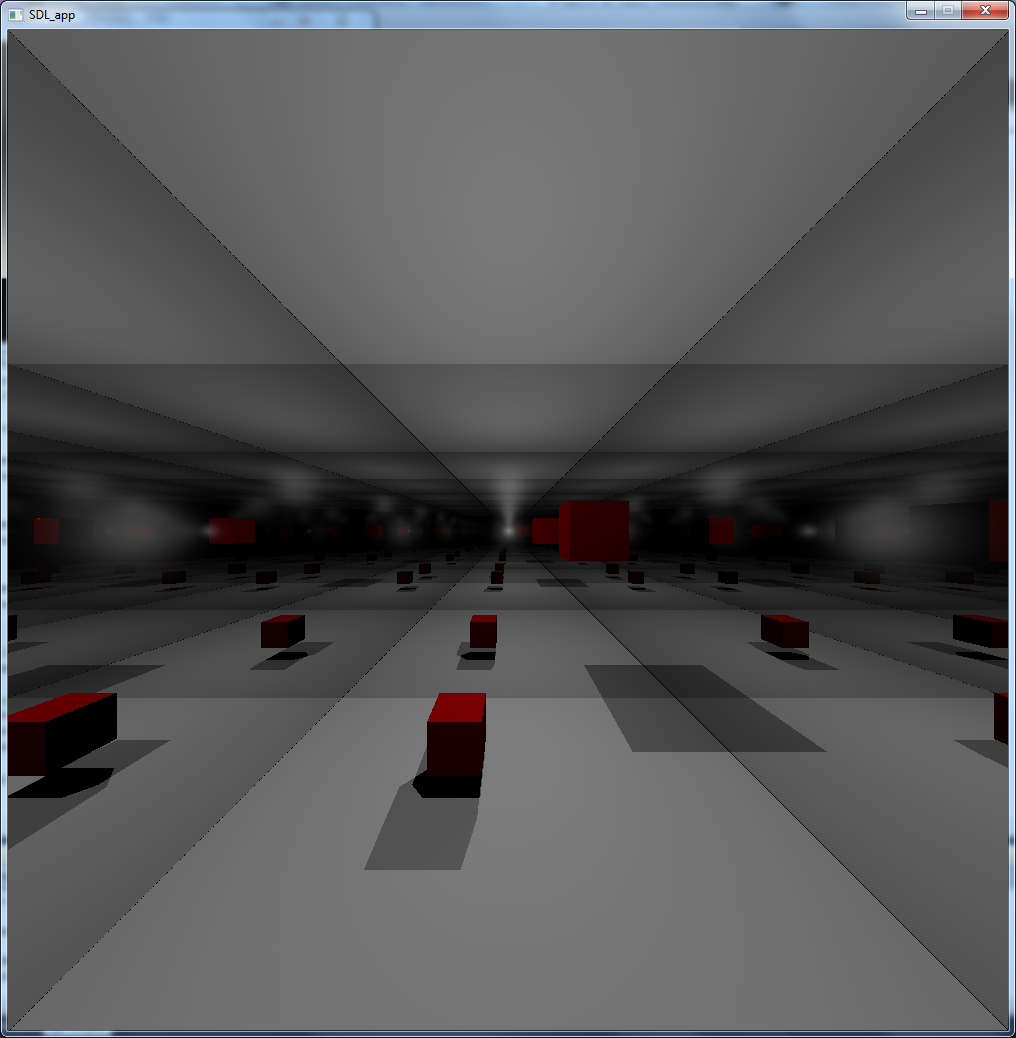
\includegraphics[width=1.00\textwidth]{img/p15.png}
    \caption{Résultat du lancé de rayon, avec une récursivité max = 15}
    \label{result}
\end{figure}

\section{Amélioration}
\subsection{Réfraction}
La réfraction permet de rendre un matériau transparent en déformant la direction du rayon le traversant (effet optique
propre au changement de milieux). Nous n'avons pas réalisé cette amélioration, cependant, pour l'implémenter il
suffirai d'utiliser la récursivité de \textit{sendRay} avec un nouveau rayon (déformé en respectant les propriété du
matériau).

\subsection{BoundingBox}
Pour accélérer le calcul des intersections de la scène, on peut d'abord détecter les intersection avec des objets
simplifiés appelés bounding boxes. Même si elles sont implémenté dans le code, nous ne les avons pas prises en compte
. La scène de test est composé de trois objets seulement. Et ils sont cubiques (forme la plus simple possible\ldots).
% glossy reflection
% bounding box
\subsection{Glossy reflection}
La réflectance obtenue dans notre implémentation est parfaite. Pour imiter un matériau imparfait il faudrait que les
reflets soit plus ou moins déformés en fontion de la distance du reflet. Le calcul théorique est cependant très lourd. 
À chaque point de reflection il faut lancer un cône, soit plusieurs rayons et les moyenner.

Nous avons tenté d'approcher ce genre de résultat en lançant un nombre fixé de rayons dévié aléatoirement. Le paramètre pour
activer cet effet est l'entier \textit{glossyReflection} qui contrôle jusqu'à quelle niveau de récursion l'effet est
calculé. Nos résultats sont visibles figure \ref{glossy1} et \ref{glossy2} page \pageref{glossy1} et \pageref{glossy2}. 
\begin{figure}[!ht]
    \center
    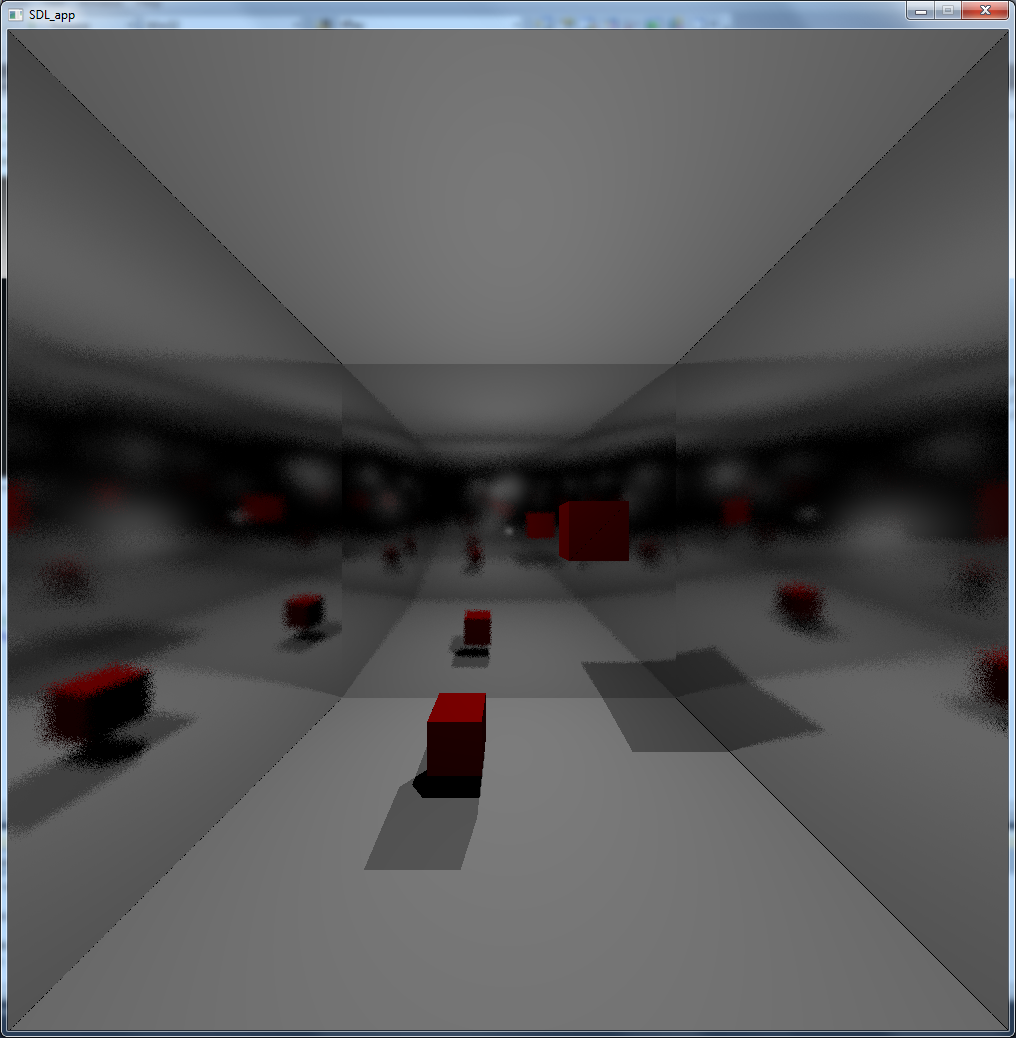
\includegraphics[width=1.00\textwidth]{img/p5mc.png}
    \caption{Approche d'une réflectance <<glossy>> avec 4 rayons réfléchis et une forte déformation}
    \label{glossy1}
\end{figure}
\begin{figure}[!ht]
    \center
    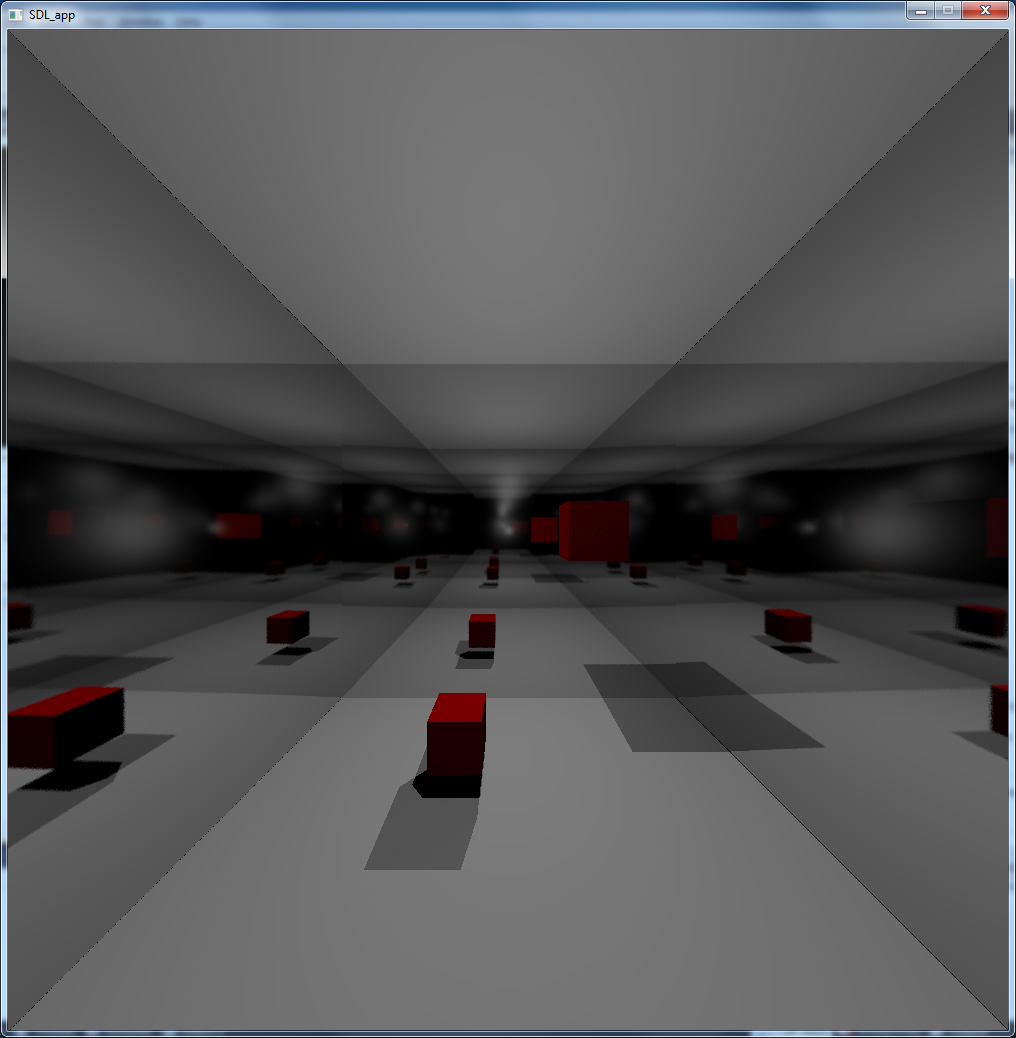
\includegraphics[width=1.00\textwidth]{img/p5mc4.png}
    \caption{Approche d'une réflectance <<glossy>> avec 14 rayons réfléchis et une faible déformation}
    \label{glossy2}
\end{figure}

Ceci est une approche
empirique, en étudiant les images obtenues, on peut remarquer des déformations trop importantes dans certaines
directions (déviation des droites, il faudrait vérifier et corriger la façons dont on dévie les rayons réfléchis), mais le reflet obtenu est quand même de plus en plus diffus en fonction de la
distance.
% éclairage ambiant diffus
\subsection{Éclairage ambiant diffus}

Pour augmenter le niveau de réalisme de la scène, on devrait pouvoir calculer l'éclairement issus des faces éclairées
des autres objets de la scène. On pourrait approcher cet effet en s'inspirant de l'amélioration précédente, mais les
temps de calculs seraient exponentiels\ldots

\section{Conclusion}
Notre implémentation permet d'obtenir le rendu d'une scène 3D en respectant les algorithmes simples tels que le
calcul des ombres, Phong et la réflectance. Notre méthode est implémenté en effectuant le moins de copies possible
et en respectant la libération mémoire des objets plus utilisés, ce qui nous permet des rendus rapide (moins de 10 secondes pour
une image 1080x1080 pixels avec une profondeur max = 15).
\end{document}
